%
%%%%%%%%%%%%%%%%%%%%%%%%%%%%%%%%%%%%%%%%%%%%%%%%%%%%%%%%%%%%%%%%%%%%%%%%
\chapter{CIS}
%%%%%%%%%%%%%%%%%%%%%%%%%%%%%%%%%%%%%%%%%%%%%%%%%%%%%%%%%%%%%%%%%%%%%%%%
%
%
\section{Launch a test}
%
%
To launch a test you must go on the CIS main page then click on your branch tab.
This will lead you to the page on Fig \ref{fig:cis-main}.
%
\begin{figure}[H]
    \centering
    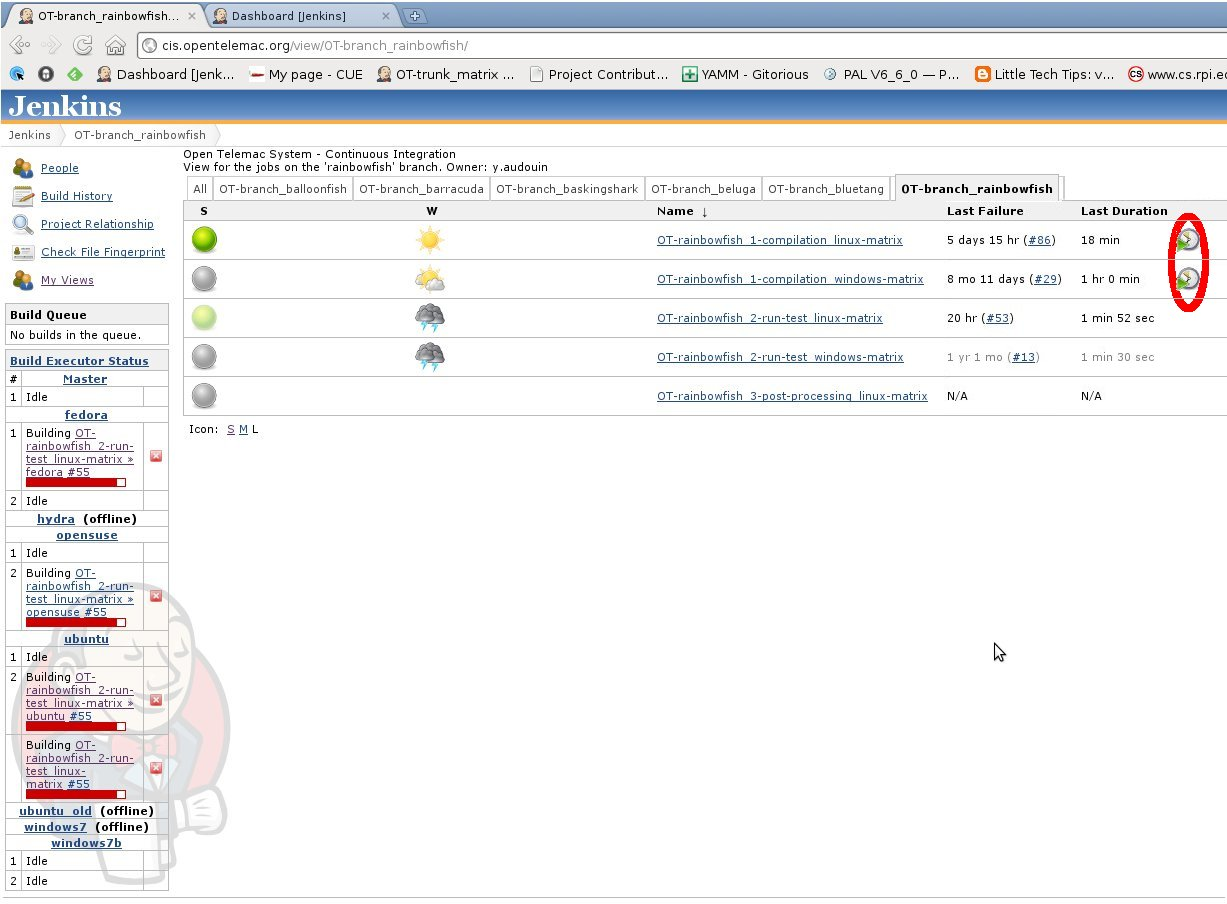
\includegraphics[scale=0.35]{graphics/cis-main.jpg}
    \caption{CIS Branch Page}
    \label{fig:cis-main}
\end{figure}
%
Click on the button in the red circle to launch the job. If you do not see that
button check that you are logged in. This will lead you to the page on Fig
\ref{fig:cis-run-job}.
%
\begin{figure}[H]
    \centering
    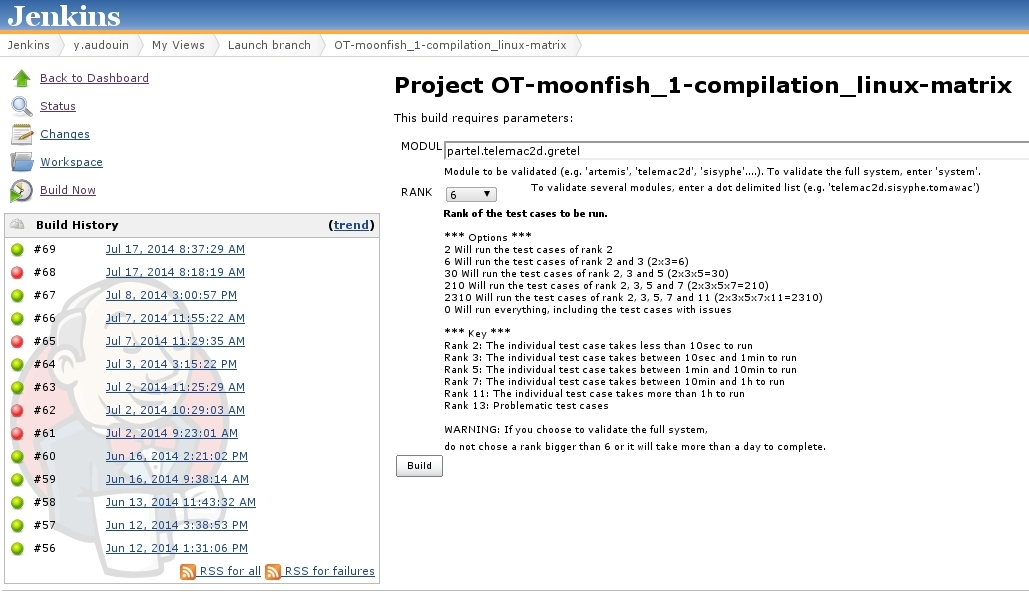
\includegraphics[scale=0.35]{graphics/cis-run-job.jpg}
    \caption{CIS Job execution}
    \label{fig:cis-run-job}
\end{figure}
%
To run the validation on your branch the following information are needed:
\begin{itemize}
\item The modules to run, if you want to run the simulation on only one module
do not forget to add partel and gretel as well to be able to run in parallel,
for exemple "partel.telemac2d.telemac3d.gretel" will run the validation on
telemac2d and telemac3d.

Writing "system" will run the validation on all the modules this is what you
need to validate a development before integration.
\item The level of complexity of test cases to run. The higher the number the
longer the test cases simulation is. For validation of a development 0 is
needed.
\end{itemize} 

If you wanna run the validation locally you need to type one the following commands:
\begin{lstlisting}[language=bash]
validateTELEMAC.py -m module
validateTELEMAC.py --ncsize=3
validateTELEMAC.py
\end{lstlisting}
The first one will launch the validate on a specify list of modules (for example
"telemac2d", "tomawac artemis").
The second one will launch the validation on the whole system but for the
parallel test cases it will replace the number of processors by 3.
The third one will run the validation on the whole system
%
%
\section{Get the listing of the test}
%
%
To see the output of the job you need to follow the step described in Fig
\ref{fig:cis-to-listing}. For step 2 you need to click on the Linux
distribution you want want to get the listing from.  For information only the
ubuntu configuration runs the test cases in parallel.
%
\begin{figure}[H]
    \centering
    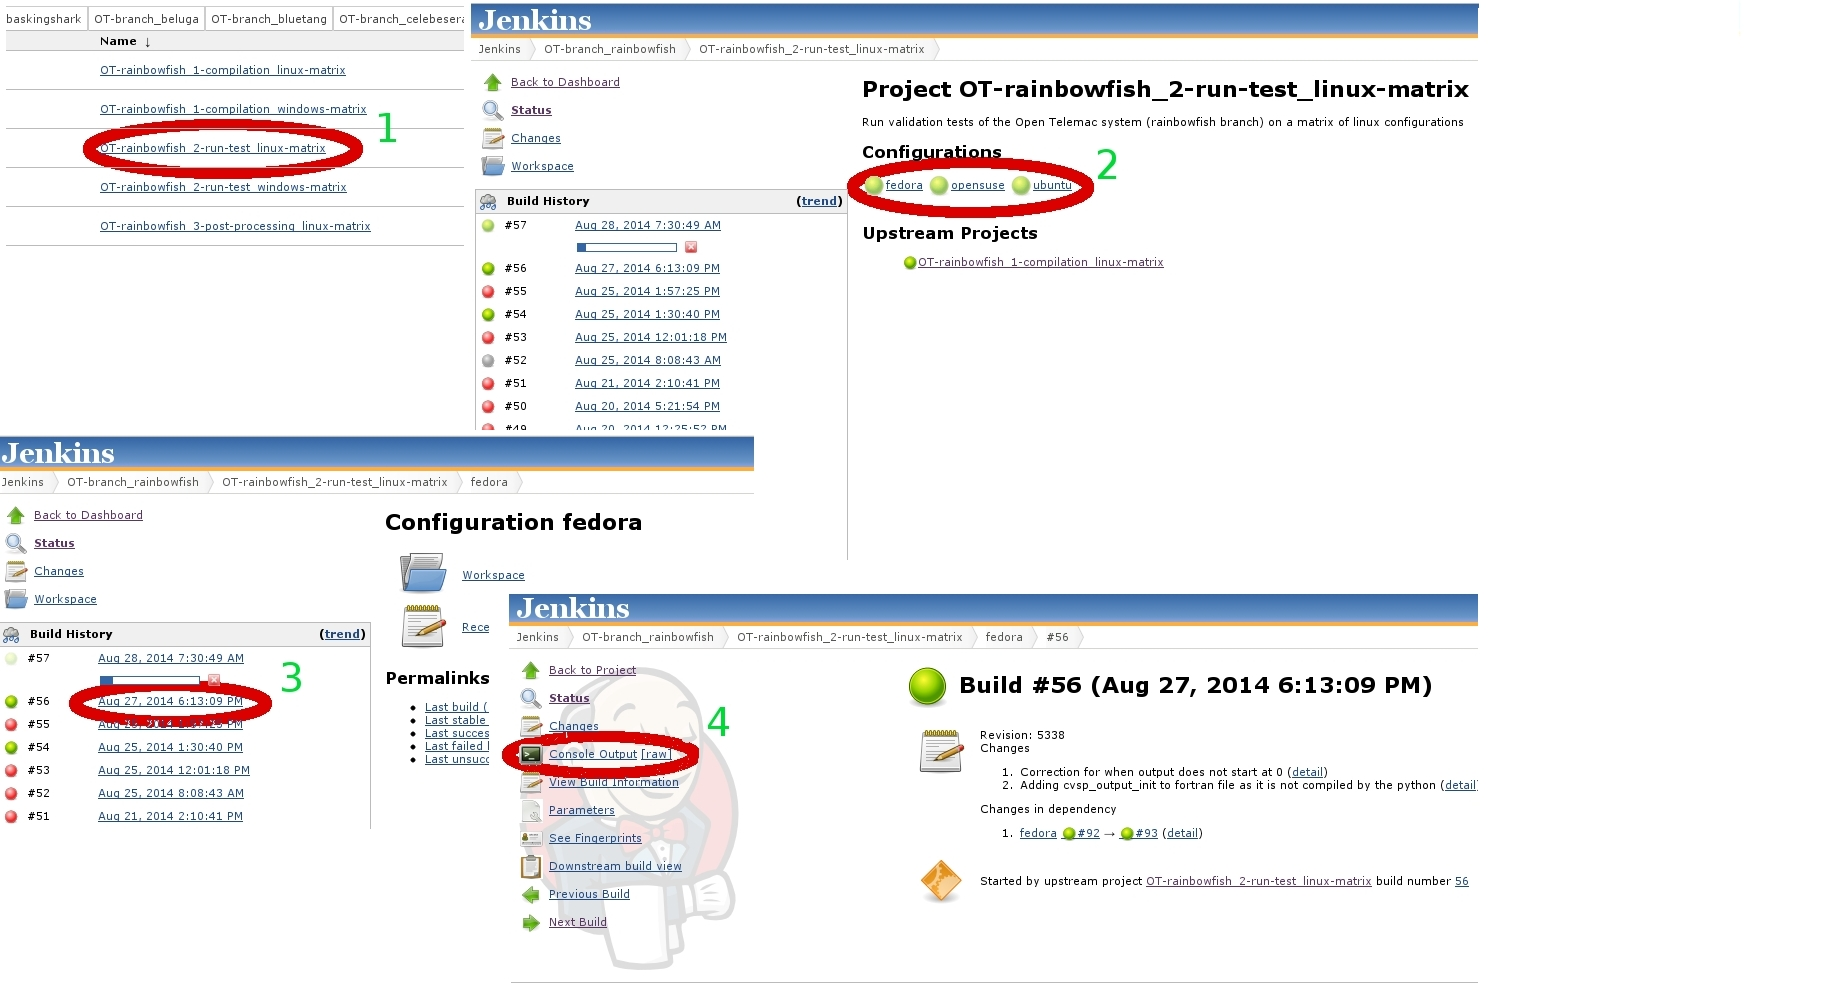
\includegraphics[scale=0.3]{graphics/cis-to-listing.jpg}
    \caption{Process to get the listing of a job execution}
    \label{fig:cis-to-listing}
\end{figure}
%
On step 4, clicking on the "raw" button will give you the complete listing as
the "Console Output" button will only give you the tail of the output that you
can see on Fig \ref{fig:cis-listing}.
%
\begin{figure}[H]
    \centering
    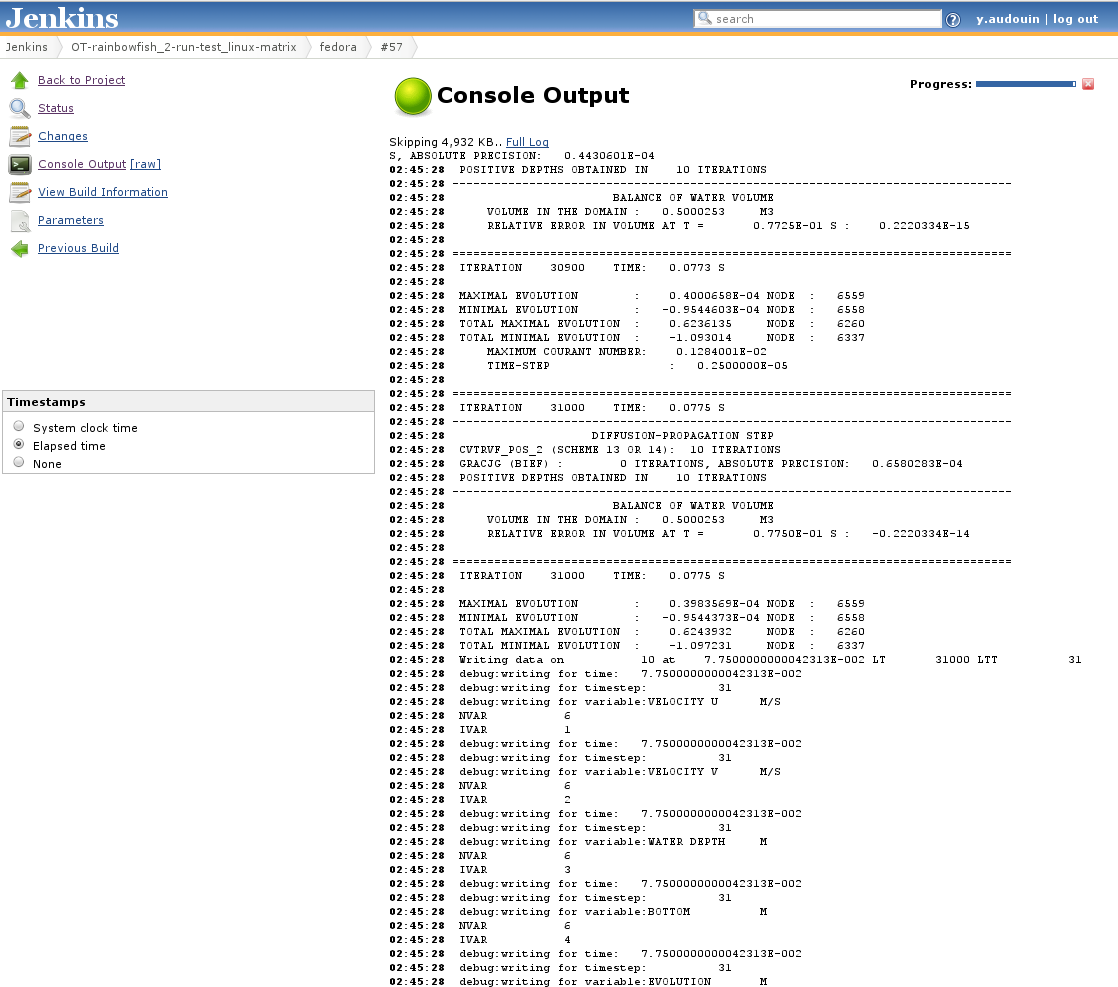
\includegraphics[scale=0.35]{graphics/cis-listing.png}
    \caption{Listing of a job execution}
    \label{fig:cis-listing}
\end{figure}
%
